% !TEX root = ../thesis.tex
%
\chapter{Evaluation}
\label{sec:evaluation}

% \cleanchapterquote{Users do not care about what is inside the box, as long as the box does what they need done.}{Jef Raskin}{about Human Computer Interfaces}

% \blindtext
% 5. Evaluation 
% (Experimental results, (1) Visualization; (2) Performance; (3) Applications)

\section{Abnormality Detection}
\label{sec:evaluation:abnormality}

The growth of smart contracts is analyzed by two types of statistics namely creation statistics and decreation statistics. Creation statistics which are associated with positive growth of smart contracts include daily number of created contracts and contract creators. Decreation statistics which are associated with negative growth of smart contracts include daily number of refund records and refunders. These statistics are visualized with time plots to detect abnormal changes.

\subsection{Creation Statistics}
\label{sec:evaluation:abnormality:creation}

\begin{table}[h]
\caption{Daily number of created contracts}
\label{tab:created-contracts}
\renewcommand\arraystretch{0.7}
\begin{tabular}{@{}cc@{}}
\toprule
\multicolumn{2}{c}{Created Contracts} \\
\midrule
Average                & 12267.14442    \\
Standard Error         & 366.8075104    \\
Median                 & 7510.5         \\
Mode                   & 7267           \\
Standard Deviation     & 11089.48345    \\
Variance               & 122976643.2    \\
Kurtosis               & 2.305335977    \\
Skewness               & 1.789698857    \\
Minimum                & 650            \\
Maximum                & 52959          \\
Summation              & 11212170       \\
Observation            & 914            \\
\bottomrule
\end{tabular}
\end{table}

From the descriptive statistics of created contracts in 914 days in Table \ref{tab:created-contracts}, the daily numbers of created contracts ranging from 650 to 52959 had a mean at 12267 and a standard deviation at 11089, the high ratio of standard deviation to mean indicated a large variation in the distribution. With reference to a normal distribution which has skewness and relative kurtosis both at 0, skewness and kurtosis measure the deviation from normal distribution in terms of degree of asymmetry and portion of outliers respectively. The daily numbers of created contracts had skewness at 1.79 and kurtosis at 2.31, its distribution was right-skewed and had low portion of outliers.

\begin{figure}[htb]
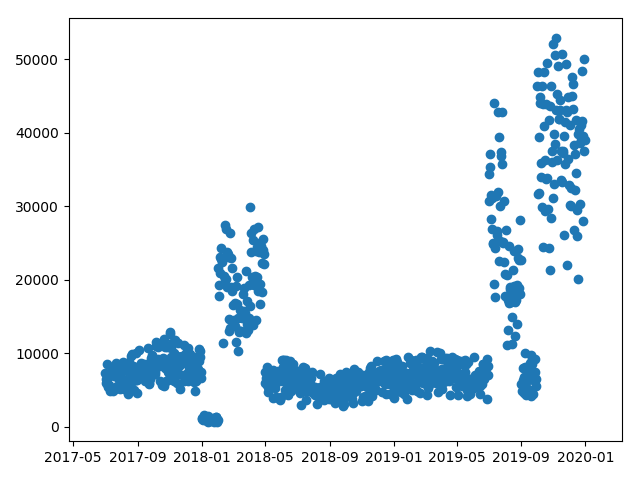
\includegraphics[width=0.7\textwidth]{gfx/created-contracts.png}
\caption{Daily number of created contracts}
\label{fig:created-contracts}
\end{figure}

From the time plot of created contracts in Fig. \ref{fig:created-contracts}, the daily numbers of created contracts had different activity levels in four time intervals. The first interval was before January 2018, the activity level was low with a flat trend. The second interval was from January to May 2018, the activity level rose sharply and reached a peak. The third interval is from June 2018 to June 2019, the activity level dropped sharply and remained a flat trend. The fourth interval was after June 2019, the activity level rose sharply and reached another peak.

\begin{table}[h]
\caption{Daily number of contract creators}
\label{tab:contract-creators}
\renewcommand\arraystretch{0.7}
\begin{tabular}{@{}cc@{}}
\toprule
\multicolumn{2}{c}{Contract Creators} \\
\midrule
Average            & 5343.724 \\
Standard   Error   & 100.7515 \\
Median             & 5278     \\
Mode               & 1474     \\
Standard Deviation & 3045.963 \\
Variance           & 9277890  \\
Kurtosis           & -1.05016 \\
Skewness           & 0.139566 \\
Range              & 12489    \\
Minimum            & 250      \\
Maximum            & 12739    \\
Summation          & 4884164  \\
Observation        & 914      \\
\bottomrule
\end{tabular}
\end{table}

From the descriptive statistics of contract creators in Table \ref{tab:contract-creators}, the daily numbers of contract creators ranging from 250 to 12739 had a mean at 5344 and a standard deviation at 3046, the high ratio of standard deviation to mean indicated a large variation in the distribution. The daily numbers of contract creators had skewness at 0.14 and kurtosis at -1.05, its distribution was slightly right-skewed and had moderately high portion of outliers.

\begin{figure}[htb]
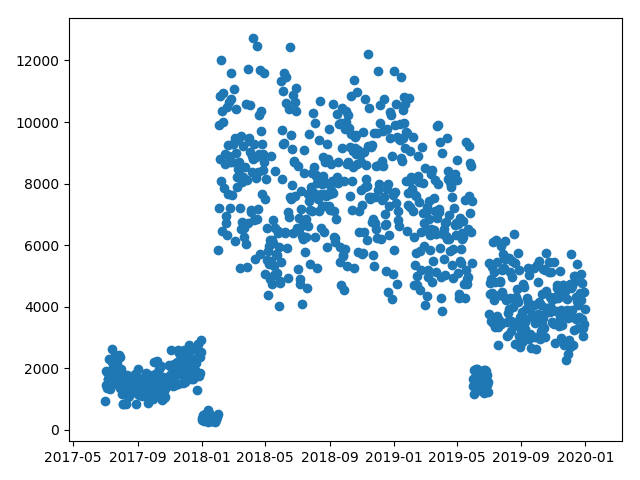
\includegraphics[width=0.7\textwidth]{gfx/contract-creators.png}
\caption{Daily number of contract creators}
\label{fig:contract-creators}
\end{figure}

From the time plot of contract creators in Fig. \ref{fig:contract-creators}, the daily numbers of contract creators had different activity levels in three time intervals. The first interval was before February 2018, the activity level was low with a flat trend. The second interval was from February 2018 to May 2019, the activity level reached a peak and fluctuated with direction. The third interval is after May 2019, the activity level dropped sharply and fluctuated without direction.

\subsection{Decreation Statistics}
\label{sec:evaluation:abnormality:decreation}

\begin{table}[h]
\caption{Daily number of refund records}
\label{tab:refund-records}
\renewcommand\arraystretch{0.7}
\begin{tabular}{@{}cc@{}}
\toprule
\multicolumn{2}{c}{Refund Records} \\
\midrule
Average                & 246067.8654    \\
Standard Error         & 9534.322429    \\
Median                 & 87599.5        \\
Mode                   & 67             \\
Standard   Deviation   & 288245.7632    \\
Variance               & 83085620024    \\
Kurtosis               & -0.193791222   \\
Skewness               & 0.953646715    \\
Range                  & 1093572        \\
Minimum                & 52             \\
Maximum                & 1093624        \\
Summation              & 224906029      \\
Observation            & 914            \\
\bottomrule
\end{tabular}
\end{table}

From the descriptive statistics of refund records in Table \ref{tab:refund-records}, the daily numbers of refund records ranging from 52 to 1093624 had a mean at 246068 and a standard deviation at 288246, the high ratio of standard deviation to mean indicated a large variation in the distribution. The daily numbers of refund records had skewness at 0.95 and kurtosis at -0.19, its distribution was moderately right-skewed and had slightly high portion of outliers.

\begin{figure}[htb]
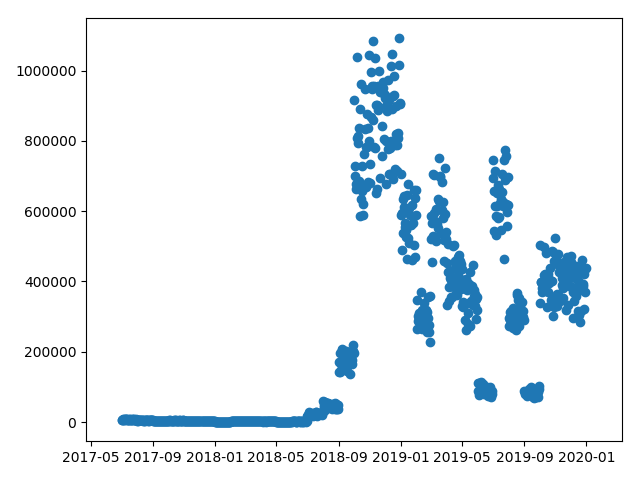
\includegraphics[width=0.7\textwidth]{gfx/refund-records.png}
\caption{Daily number of refund records}
\label{fig:refund-records}
\end{figure}

From the time plot of refund records in Fig. \ref{fig:refund-records}, the daily numbers of refund records had different activity levels in two time intervals. The first interval was before September 2018, the activity level was low with a flat trend. The second interval was after September 2018, the activity level reached a peak and fluctuated without direction.

\begin{table}[h]
\caption{Daily number of refunders}
\label{tab:refunders}
\renewcommand\arraystretch{0.7}
\begin{tabular}{@{}cc@{}}
\toprule
\multicolumn{2}{c}{Refunders} \\
\midrule
Average                       & 276.2144           \\
Standard Error                & 15.22506           \\
Median                        & 111                \\
Mode                          & 81                 \\
Standard Deviation            & 460.2905           \\
Variance                      & 211867.4           \\
Kurtosis                      & 15.55016           \\
Skewness                      & 3.759675           \\
Range                         & 3169               \\
Minimum                       & 5                  \\
Maximum                       & 3174               \\
Summation                     & 252460             \\
Observation                   & 914                \\
\bottomrule
\end{tabular}
\end{table}

From the descriptive statistics of refunders in Table \ref{tab:refunders}, the daily numbers of refunders ranging from 5 to 3174 had a mean at 276 and a standard deviation at 460, the high ratio of standard deviation to mean indicated a large variation in the distribution. The daily numbers of refunders had skewness at 3.76 and kurtosis at 15.55, its distribution was right-skewed and had low portion of outliers.

\begin{figure}[htb]
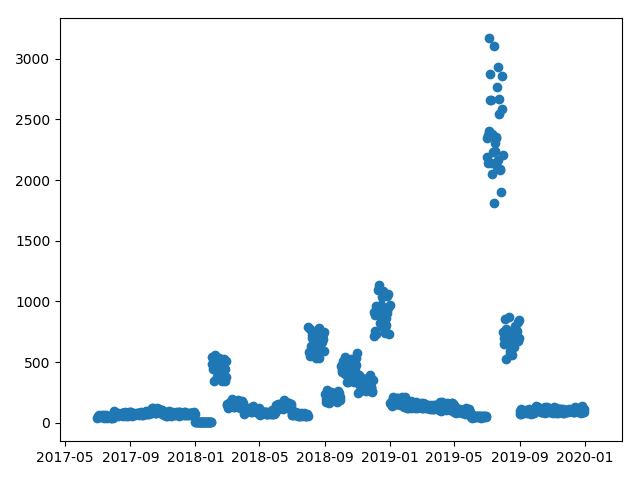
\includegraphics[width=0.7\textwidth]{gfx/refunders.png}
\caption{Daily number of refunders}
\label{fig:refunders}
\end{figure}

From the time plot of refunders in Fig. \ref{fig:refunders}, the daily numbers of refunders had different activity levels in three time intervals. The first interval was before July 2019, the activity level was low and flucuated without direction. The second interval was from July to September 2019, the activity level rose sharply and reached a peak. The third interval was after September 2019, the activity level dropped sharply and remained a flat trend.

\subsection{Significant Event}
\label{sec:evaluation:abnormality:event}

From the descriptive statistics of smart contract growth in section \ref{sec:evaluation:abnormality:creation} and section \ref{sec:evaluation:abnormality:decreation}, 2018 was a special year when abnormal changes in activity level took place. Around this year, there was a significant event in Ethereum blockchain, the issuance of a stable currency called Dai.

At the end of 2017, Dai built by Maker Foundation was issued as an ERC-20 token. Unlike Bitcoin which has volatile value and acts more like an investment than cash, Dai is marketed as a digital version of real money and its value consistently tracks the USD. To maintain stable value relative to USD, it is backed by assets which value is locked in publicly viewable smart contracts and adjusted automatically by algorithm. By removing the volatility of a typical cryptocurrency, Dai can store and exchange value like traditional money to serve many financial applications such as spending and lending, this can be a reason that activity level of smart contracts increased sharply for 2018.

\section{Impact Analysis}
\label{sec:evaluation:impact}

% \blindtext
In 2018 after the stable coin Dai was issued, the activities of exchanges including money transfer, smart contract creation, smart contract invocation could partially reflect the distribution of its impact. For example, the CIG representing contract invocation activities of decentralized exchanges can be further analyzed as decentralized exchanges had much less activities in money transfer and smart contract creation in 2018. To be clear, the exchanges are classified as decentralized exchanges in the exchange directory on EtherScan \cite{17}.

\begin{figure}[htb]
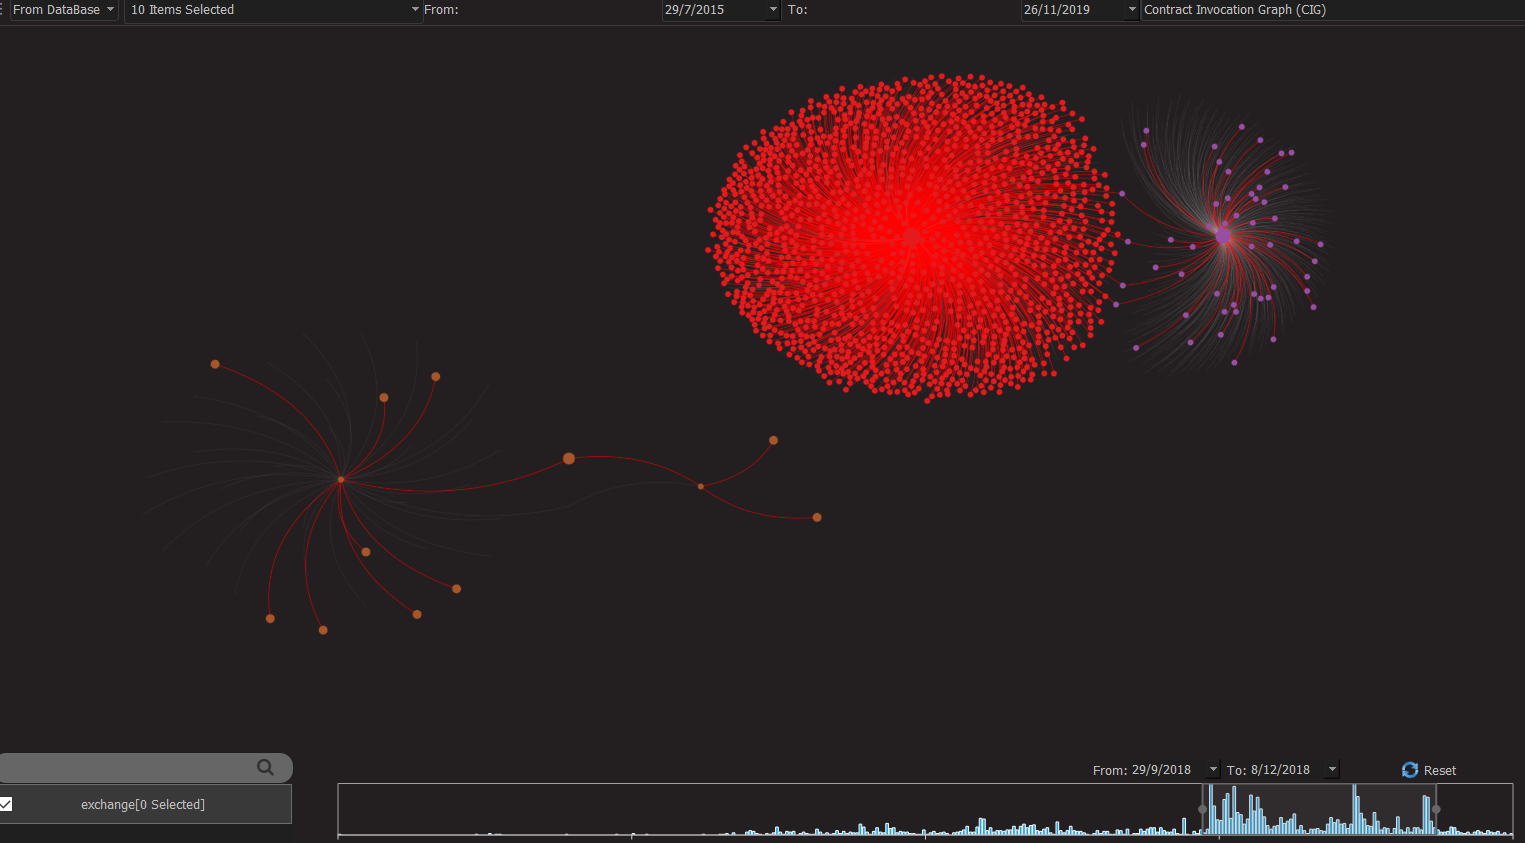
\includegraphics[width=\textwidth]{gfx/impact-analysis.png}
\caption{CIG of decentralized exchanges in selected interval}
\label{fig:impact-analysis}
\end{figure}

In the selected time interval covering highest activity levels in smart contract invocation by decentralized exchanges in 2018, Fig. \ref{fig:impact-analysis} illustrates the distribution of contribution to these activity levels for different exchanges. Among them, the decentralized exchange "Allbit" as a contract had most transactions associated with it. During this period from Oct 2018 to Dec 2018, "Allbit" introduced Dai coin into its products on 12 Oct \cite{22}. It was probably one of the reasons to attract high contract invocation activity in this period. 

\section{Evolutionary Study}
\label{sec:evaluation:evolution}

% \blindtext
One focus of evolutionary study is to analyze the growth of an individual in terms of its importance and relationships with other parties. In Fig. \ref{fig:impact-analysis} it shows that "Allbit" contributed the highest transaction volume in smart contract invocation among decentralized exchanges in 2018, it is worth noting that it was also launched in 2018. Therefore, the CIG in four incremental time intervals are visualized to analyze the changes of its importance and relationships with others.

\begin{figure}[htb]
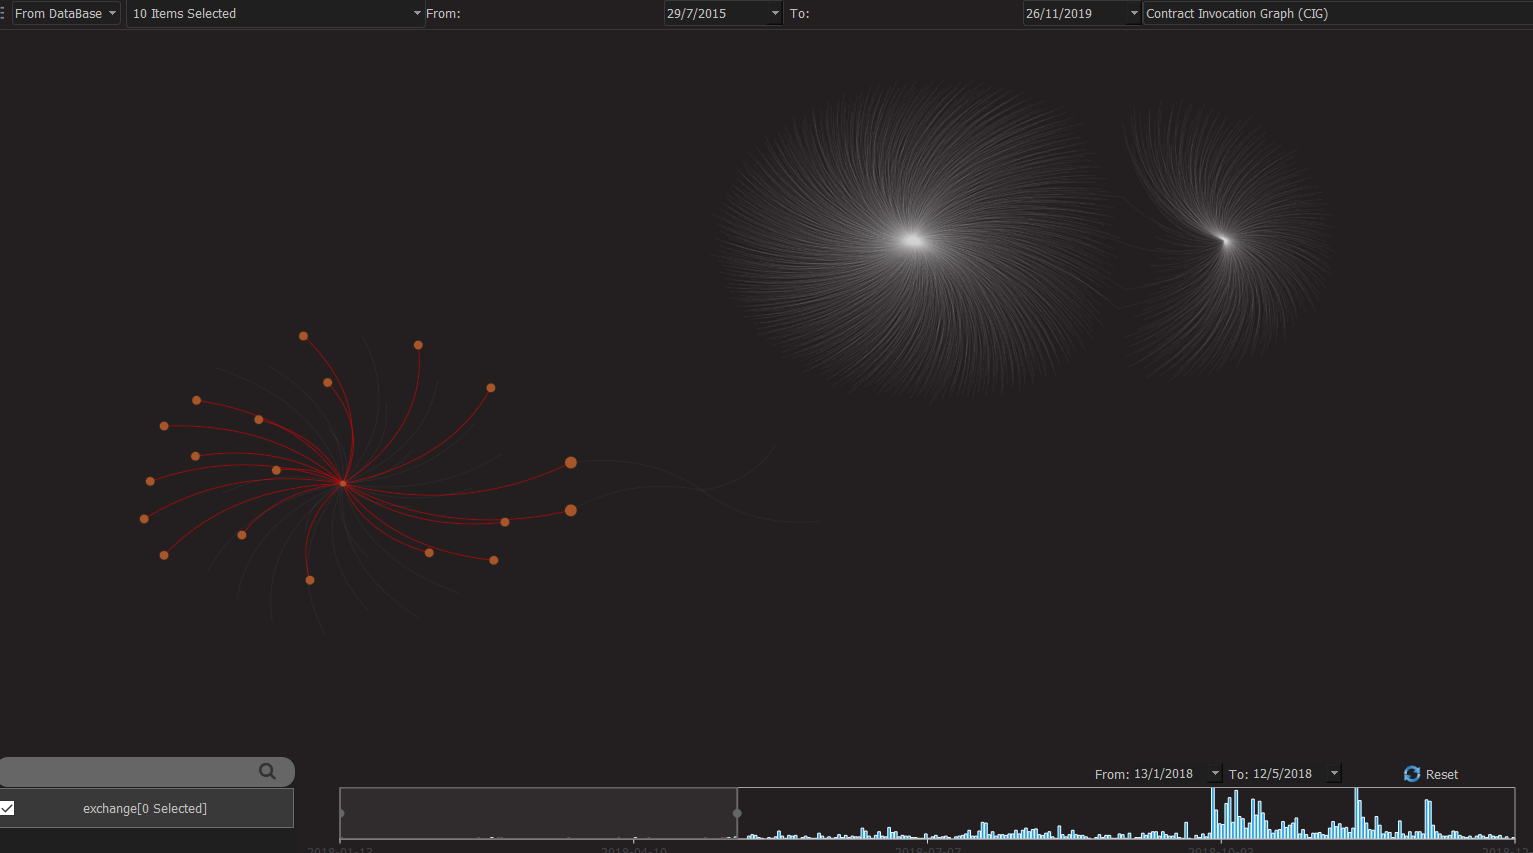
\includegraphics[width=0.7\textwidth]{gfx/evolutionary-study1.png}
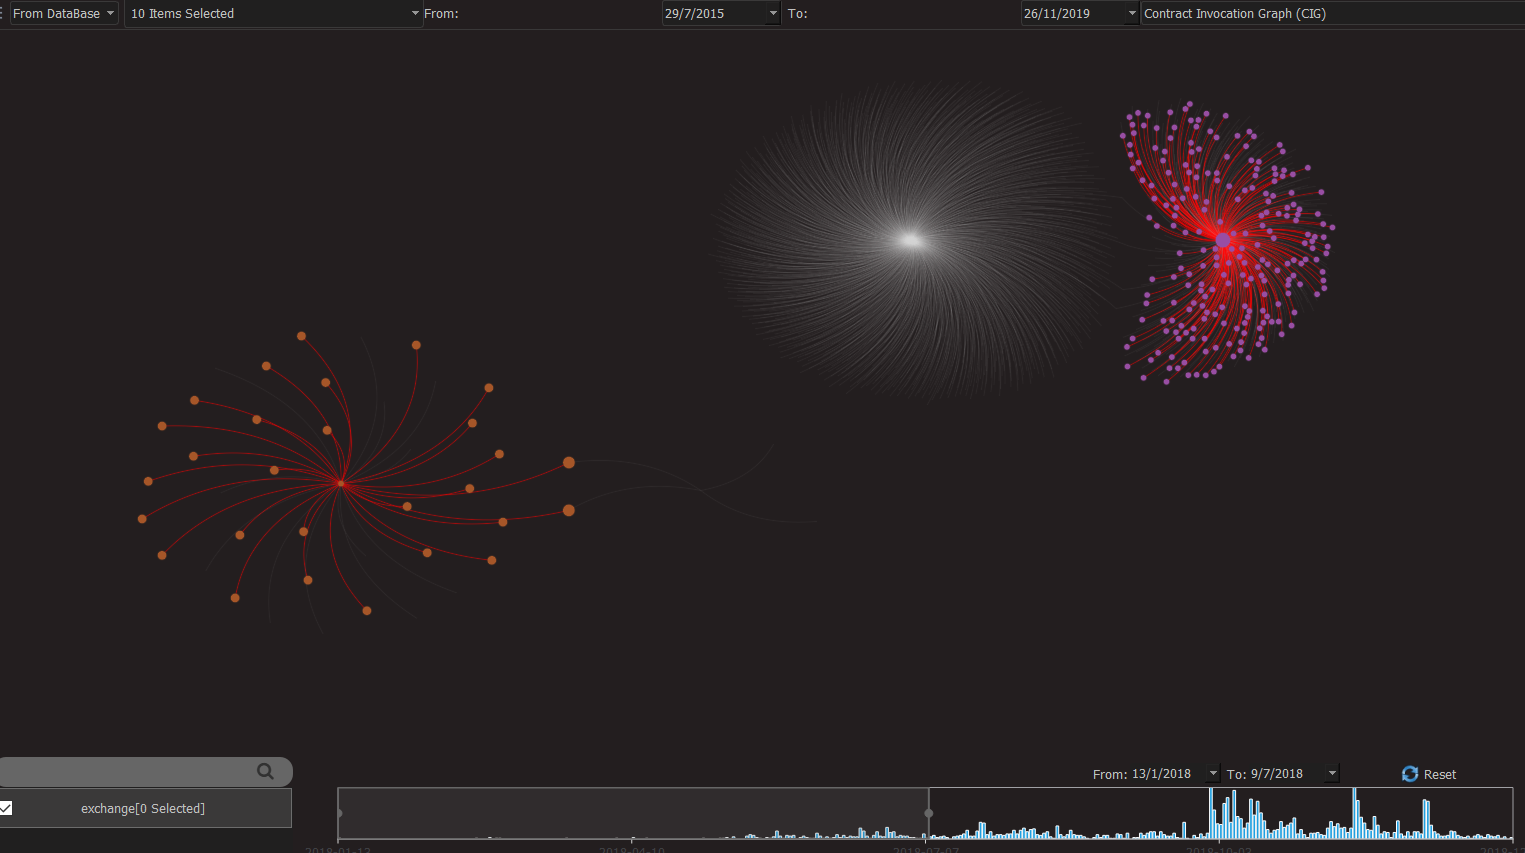
\includegraphics[width=0.7\textwidth]{gfx/evolutionary-study2.png}
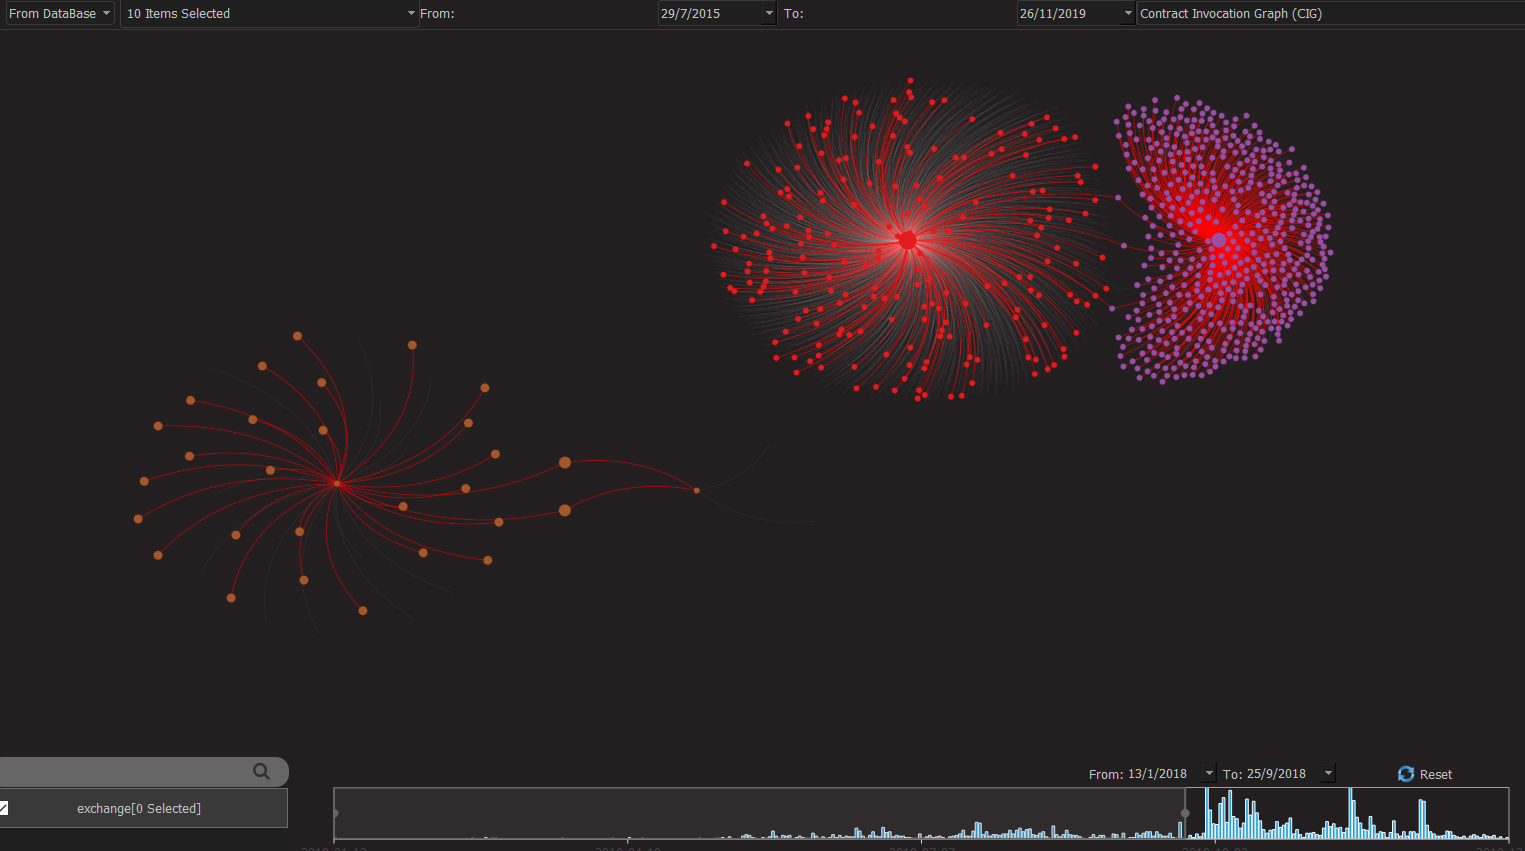
\includegraphics[width=0.7\textwidth]{gfx/evolutionary-study3.png}
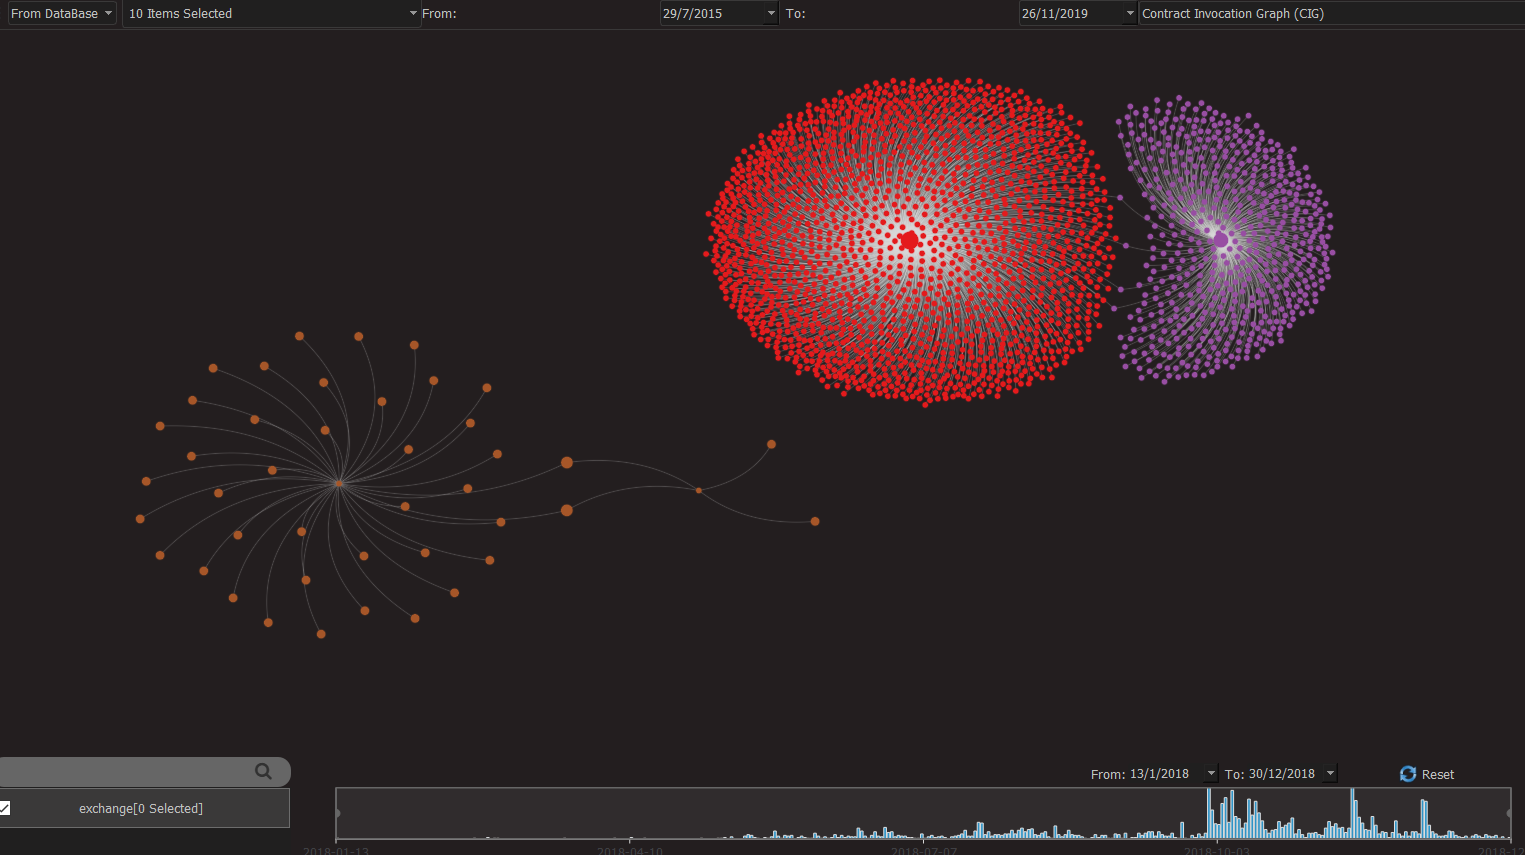
\includegraphics[width=0.7\textwidth]{gfx/evolutionary-study4.png}
\caption{CIG of decentralized exchanges in incremental intervals}
\label{fig:evolutionary-study}
\end{figure}

From Fig. \ref{fig:evolutionary-study}, "Allbit" gained the highest degree centrality and formed the largest Louvain community among decentralized exchanges in 2018. "Allbit" was launched after the launch of "DEx.top" when "DEx.top" had certain degree of market share at that moment, then "Allbit" grew at a much higher speed than "Dex.top", eventually "Allbit" exceeded its competitor "DEx.top" in centrality and community measures after adding Dai currency as its product. In Fig. \ref{fig:impact-analysis}, it can also be observed that when "Allbit" reached peak transaction volume, "DEx.top" only had little growth \cite{23}.


% \section{Summary}
% \label{sec:real:summary}

% \blindtext
